\documentclass[a4paper, 12pt]{report}
\usepackage{hyperref}
\usepackage{gensymb}
\usepackage{ amssymb }
\usepackage[utf8]{inputenc} % выбор кодировки кода
\usepackage[T2A]{fontenc} % выбор внутренней кодировки 
\usepackage[english, russian]{babel} % выбор языка
\usepackage{csquotes}
% \righthyphenmin = 2 % минимальное число букв после переноса: может пригодиться
\usepackage{multirow}
\usepackage{fontawesome}
\usepackage{easyReview}
\usepackage{tabularx}
\usepackage{rotating}
\usepackage{amsmath} % русский текст в формулах
\usepackage{color} % цвет текста
\usepackage{ulem} % для зачёркивания текстаё

\usepackage[left=15mm, right=10mm, top=20mm, bottom=20mm]{geometry} % поля
\usepackage{indentfirst} % отступ первого абзаца
\setlength{\parindent}{1,25cm} % длина отступа первой строки абзаца
\linespread{1,5} % междустрочный интервал

\usepackage{titlesec} % настройка заголовков
\renewcommand{\thesection}{\arabic{section}} % противотараканная мера для report'а: делаю section заголовком первого уровня
\titleformat{\section}{\centering \large \bfseries}{\thesection}{1ex}{\MakeUppercase}{}
\titleformat{\subsection}{\centering \large \bfseries}{\thesubsection}{1ex}{}{}
\titleformat{\subparagraph}[runin]{\bfseries}{\thesubparagraph}{}{}{}

% \titleformat{\bibliography}{\centering \large \bfseries}{\thebibliography}{}{}{} % попытка настроить заголовок для списка литературы

\usepackage{graphicx}
\usepackage{wasysym}

\usepackage{comment} % Для многострочных комментариев
\usepackage{xcolor} % Для девочек 
\usepackage{enumitem} 
\usepackage{wasysym} % Для смайликов

\usepackage[
natbib		= true,
style		= gost-numeric,
sorting		= none,
backend		= biber,
language	= autobib,
bibstyle	= gost-numeric,
citestyle	= gost-numeric,
autolang	= other]{biblatex}
\addbibresource{mybiblio.bib}

\usepackage{xstring} % Для преподов
% Команда для вставки изображения из google drive по ссылке
\newcounter{imagecounter}
\setcounter{imagecounter}{0}

\newcommand{\includegoogle}[2][]{%
	\stepcounter{imagecounter}%
	\edef\tempfilename{temp-image-\theimagecounter.jpg}% % Создаем уникальное имя
	
	% #1 - опции изображения (width, height и т.д.)
	% #2 - ссылка на Google Drive
	% #3 - заголовок (caption)
	
	% Извлекаем ID
	\StrBehind{#2}{/file/d/}[\tempurl]%
	\StrBefore{\tempurl}{/}[\fileid]%
	\StrBehind{#2}{id=}[\tempurlb]%
	\StrBefore{\tempurlb}{&}[\fileidb]%
	
	\IfStrEq{\fileid}{}{%
		\IfStrEq{\fileidb}{}{%
			\def\finalid{#2}%
		}{%
			\def\finalid{\fileidb}%
		}%
	}{%
		\def\finalid{\fileid}%
	}%
	
	\immediate\write18{curl -s -L -o "\tempfilename" "https://drive.google.com/uc?export=download&id={\finalid}"}%
	
	\IfFileExists{\tempfilename}{%
		\includegraphics[#1]{\tempfilename}
	}{%
		\fbox{\parbox{0.8\textwidth}{\centering\textcolor{red}{Error}\\Link: #2\\ID: \finalid}}%
	}%
	
%	\AtEndDocument{%
%		\forlistloop{\immediate\write18{del "#1" 2>nul}}{\tempfileslist}%
%	}
	
%	% Удаляем конкретный временный файл в конце
%	\AtEndDocument{%
%		\immediate\write18{del "\tempfilename" 2>nul}%
%	}%
}

\begin{document}
	%%%%%%%%%%%%%%%%%%%%%%%%%%%%%
	% Как вставлять картинки?
	%%%%%%%%%%%%%%%%%%%%%%%%%%%%%
	% В TexStudio в Параметры -> Команды -> PdLaTeX должно быть написано smth -shell-escape %.tex
	% Как работать в других редакторах - не знаю, но если есть идеи - дополняйте!
	% 	\includegoogle[width=0.8\textwidth]{ссылка на изображение с google drive - оно должно быть открыто для просмотра}{Подпись к картинке}
	%%%%%%%%%%%%%%%%%%%%%%%%%%%%%
	
	\begin{titlepage}
\setlength\parindent{0pt}
	\begin{center}
		\large{РОО <<Федерация спортивного туризма Московской области>>\\
		ОО г. Долгопрудного <<Федерация спортивного туризма>>\\}
	\end{center}

	


	
	\begin{center}
		\includegraphics[width=0.4\linewidth]{pics/Flag_GS-2}
		
		\Large{\bfseries{ОТЧЁТ}} \\
		\normalsize о прохождении пешеходного спортивного туристического маршрута \textbf{первой} категории сложности по Кавказу, Приэльбрусье, совершённом с 05 по 11 сентября 2025 г. группой туристов Горной секции МФТИ ФСТ Московской области, г. Долгопрудный
	\end{center}
	\vspace{1.5 cm}
	
	\textbf{Маршрутная книжка:} 94/2025, выдана МКК ФСТ МО г. Долгопрудный \\ 
	\textbf{Руководитель группы:} Остапив Алексей Юрьевич\\
	\textbf{E-mail:} \href{mailto: ostapiv\_ayu@phystech.edu}{ostapiv\_ayu@phystech.edu}\\
	\textbf{Номер телефона:} $+7(989)629-46-58$
	
	\vspace{0.2cm}
	
	\textit{Маршрутно-квалификационная комиссия Федерации спортивного туризма Московской области рассмотрела отчёт и считает, что маршрут может быть зачтён всем участникам и руководителю \textbf{первой категории сложности}.}

	\vspace{0.2cm}
	
	Отчёт использовать в библиотеке ФСТ Московской области и ФСТ г. Долгопрудный.
	
	\vspace{0.8cm}
	\textbf{Судья по виду:} 
	
%	\vspace{0.8cm}
%	\textbf{Судья по ходу:}
	
	\vspace{0.8cm}
	\textbf{Председатель МКК:}
	
	\vspace{0.8cm}
	\textbf{Штамп МКК:}
	
	\vfill
	\begin{center}
		Долгопрудный,   \the\year{}
	\end{center}
\end{titlepage}
	\input{contents}
	\section*{Сокращения, используемые в отчёте}
\addcontentsline{toc}{section}{Сокращения, используемые в отчёте}
\begin{table}[h!]
\centering
\begin{tabular}{p{0.08\textwidth} p{0.4\textwidth} | p{0.08\textwidth} p{0.4\textwidth}}
	МКК                                  &   Маршрутно-квалификационная комиссия  &	кырг.	&	Кыргызский (язык)	\\
	ФСТ                                &   Федерация спортивного туризма  & м.н. & место ночёвки \\
	к.с.                               &   категория сложности (похода) & 
	ст.с.							& степень сложности (похода) \\
	н/к                            &   некатегорированный (перевал, препятствие) &	орогр.                &   орографически \\
	рук. &   руководитель &а/л                  &   альпинистский лагерь  \\
	ЧХВ                          &   чистое ходовое время  &пхд	&	по ходу движения \\
	ОХВ                          &   общее ходовое время  & лев.	& левый \\
	т/б                         &   туристическая база & пр. &   правый \\
	т/к                         &   туристический клуб &  &    \\
		с. & село & & \\
	г. & город & & \\
	верш.               &   вершина & & \\
	пер.               &   перевал & & \\
	оз.             &   озеро & & \\
	р.             &   река & & \\
	д.	&	долина & &\\
	хр. &   хребет& & \\
	тр. &   травянистый & &\\
	ос. &   осыпной& & \\
	ск. &   скальный & &\\
	сн. &   снежный & &\\
	лед. &   ледовый & &\\	
\end{tabular}
\end{table}
\clearpage
	\section{Справочные сведения о походе} 
\subsection{Проводящая организация}
Горная секция МФТИ, г.о. Долгопрудный


\subsection{Место проведения}
\textbf{Страна:} Россия

\textbf{Субъекты федерации:} КЧР, КБР

\textbf{Район:} Западный, Центральный Кавказ

\textbf{Подрайон:} Приэльбрусье


\subsection{Общие справочные сведения о маршруте}

\begin{table}[h!]
	\resizebox{\textwidth}{!}{%
		\begin{tabular}{|c|c|c|cc|c|}
			\hline
			\multirow{2}{*}{\begin{tabular}[c]{@{}c@{}}Дисциплина\\ (вид туризма)\end{tabular}} & \multirow{2}{*}{\begin{tabular}[c]{@{}c@{}}Категория сложности\\ маршрута\end{tabular}} & \multirow{2}{*}{\begin{tabular}[c]{@{}c@{}}Протяжённость\\ активной части, км$^1$\end{tabular}} & \multicolumn{2}{c|}{\begin{tabular}[c]{@{}c@{}}Продолжительность активной\\ части\end{tabular}} & \multirow{2}{*}{Срок проведения}                                   \\ \cline{4-5}
			&                                                                                         &                                                                                             & \multicolumn{1}{c|}{Общая}                            & Ходовых дней                            &                                                                     \\ \hline
			Пешеходный                                                                              & Первая                                                                                  & 92.0                                                                                         & \multicolumn{1}{c|}{7}                               & 7                                      & \begin{tabular}[c]{@{}c@{}}05.09.2025~--\\ 11.09.2025 г.\end{tabular} \\ \hline
		\end{tabular}%
	}
\end{table}
\footnotesize{$^1$ С учётом коэффициента $k=1.1$, без учёта повторно пройденного пути}
\normalsize

\subsection{Подробная нитка маршрута}
\textbf{Заявленная:} а. Хурзук~--- д.р.~Уллу-Хурзук~--- д.р.~Еникол~--- \textbf{пер.~Енукол (н/к, 2588)}~--- \textbf{пер. Быкылы (н/к, 2963)}~--- тропа Сют-Джол~--- \textbf{пер. Чемарт (н/к, 3137)}~--- д.р.~Чемарткол~--- \textbf{пер. Бурунташ (н/к, 3072)}~--- плато Ирахитсырт~--- д.р. Кызыкол \textbf{(переправа н/к)}~--- поляна Эммануэля~--- горячие источники Джилы-Су~--- \textbf{пер. Бересун (н/к, 2450)}~--- д.р.~Исламчат~---\textbf{ пер. Кыртыкауш (н/к, 3242)}~--- д.р.~Кыртык~---\textbf{ пер. Сылтран (н/к, 3400)}~--- оз. Сылтран~--- д.р. Сылтран~--- с.~Верхний Баксан

\textbf{Пройденная:} а. Хурзук~--- д.р.~Уллу-Хурзук~--- д.р.~Еникол~--- \textbf{пер.~Енукол (н/к, 2588)}~--- \textbf{пер. Быкылы (н/к, 2963)}~--- тропа Сют-Джол~--- \textbf{пер. Чемарт (н/к, 3137)}~--- д.р.~Чемарткол~--- \textbf{пер. Бурунташ (н/к, 3072)}~--- плато Ирахитсырт~--- д.р. Кызыкол \textbf{(переправа н/к)}~--- поляна Эммануэля~--- горячие источники Джилы-Су~--- \textbf{пер. Бересун (н/к, 2450)}~--- д.р.~Исламчат~---\textbf{ пер. Кыртыкауш (н/к, 3242)}~--- д.р.~Кыртык~--- с.~Верхний Баксан

\textbf{Отличия заявленной нитки от пройденной:} отказались от прохождения пер. Сылтран и спустились по запасному варианту в Верхний Баксан. Сделали это в связи с тем, что длительный спуск (около 2 км по вертикали) почти гарантированно привёл бы к проблемам с коленями у одного из участников. К тому же, судя по отзывам встреченных нами туристов, на седловине перевала уже лежал снег.

\begin{figure}[h!tbp]
  	\centering	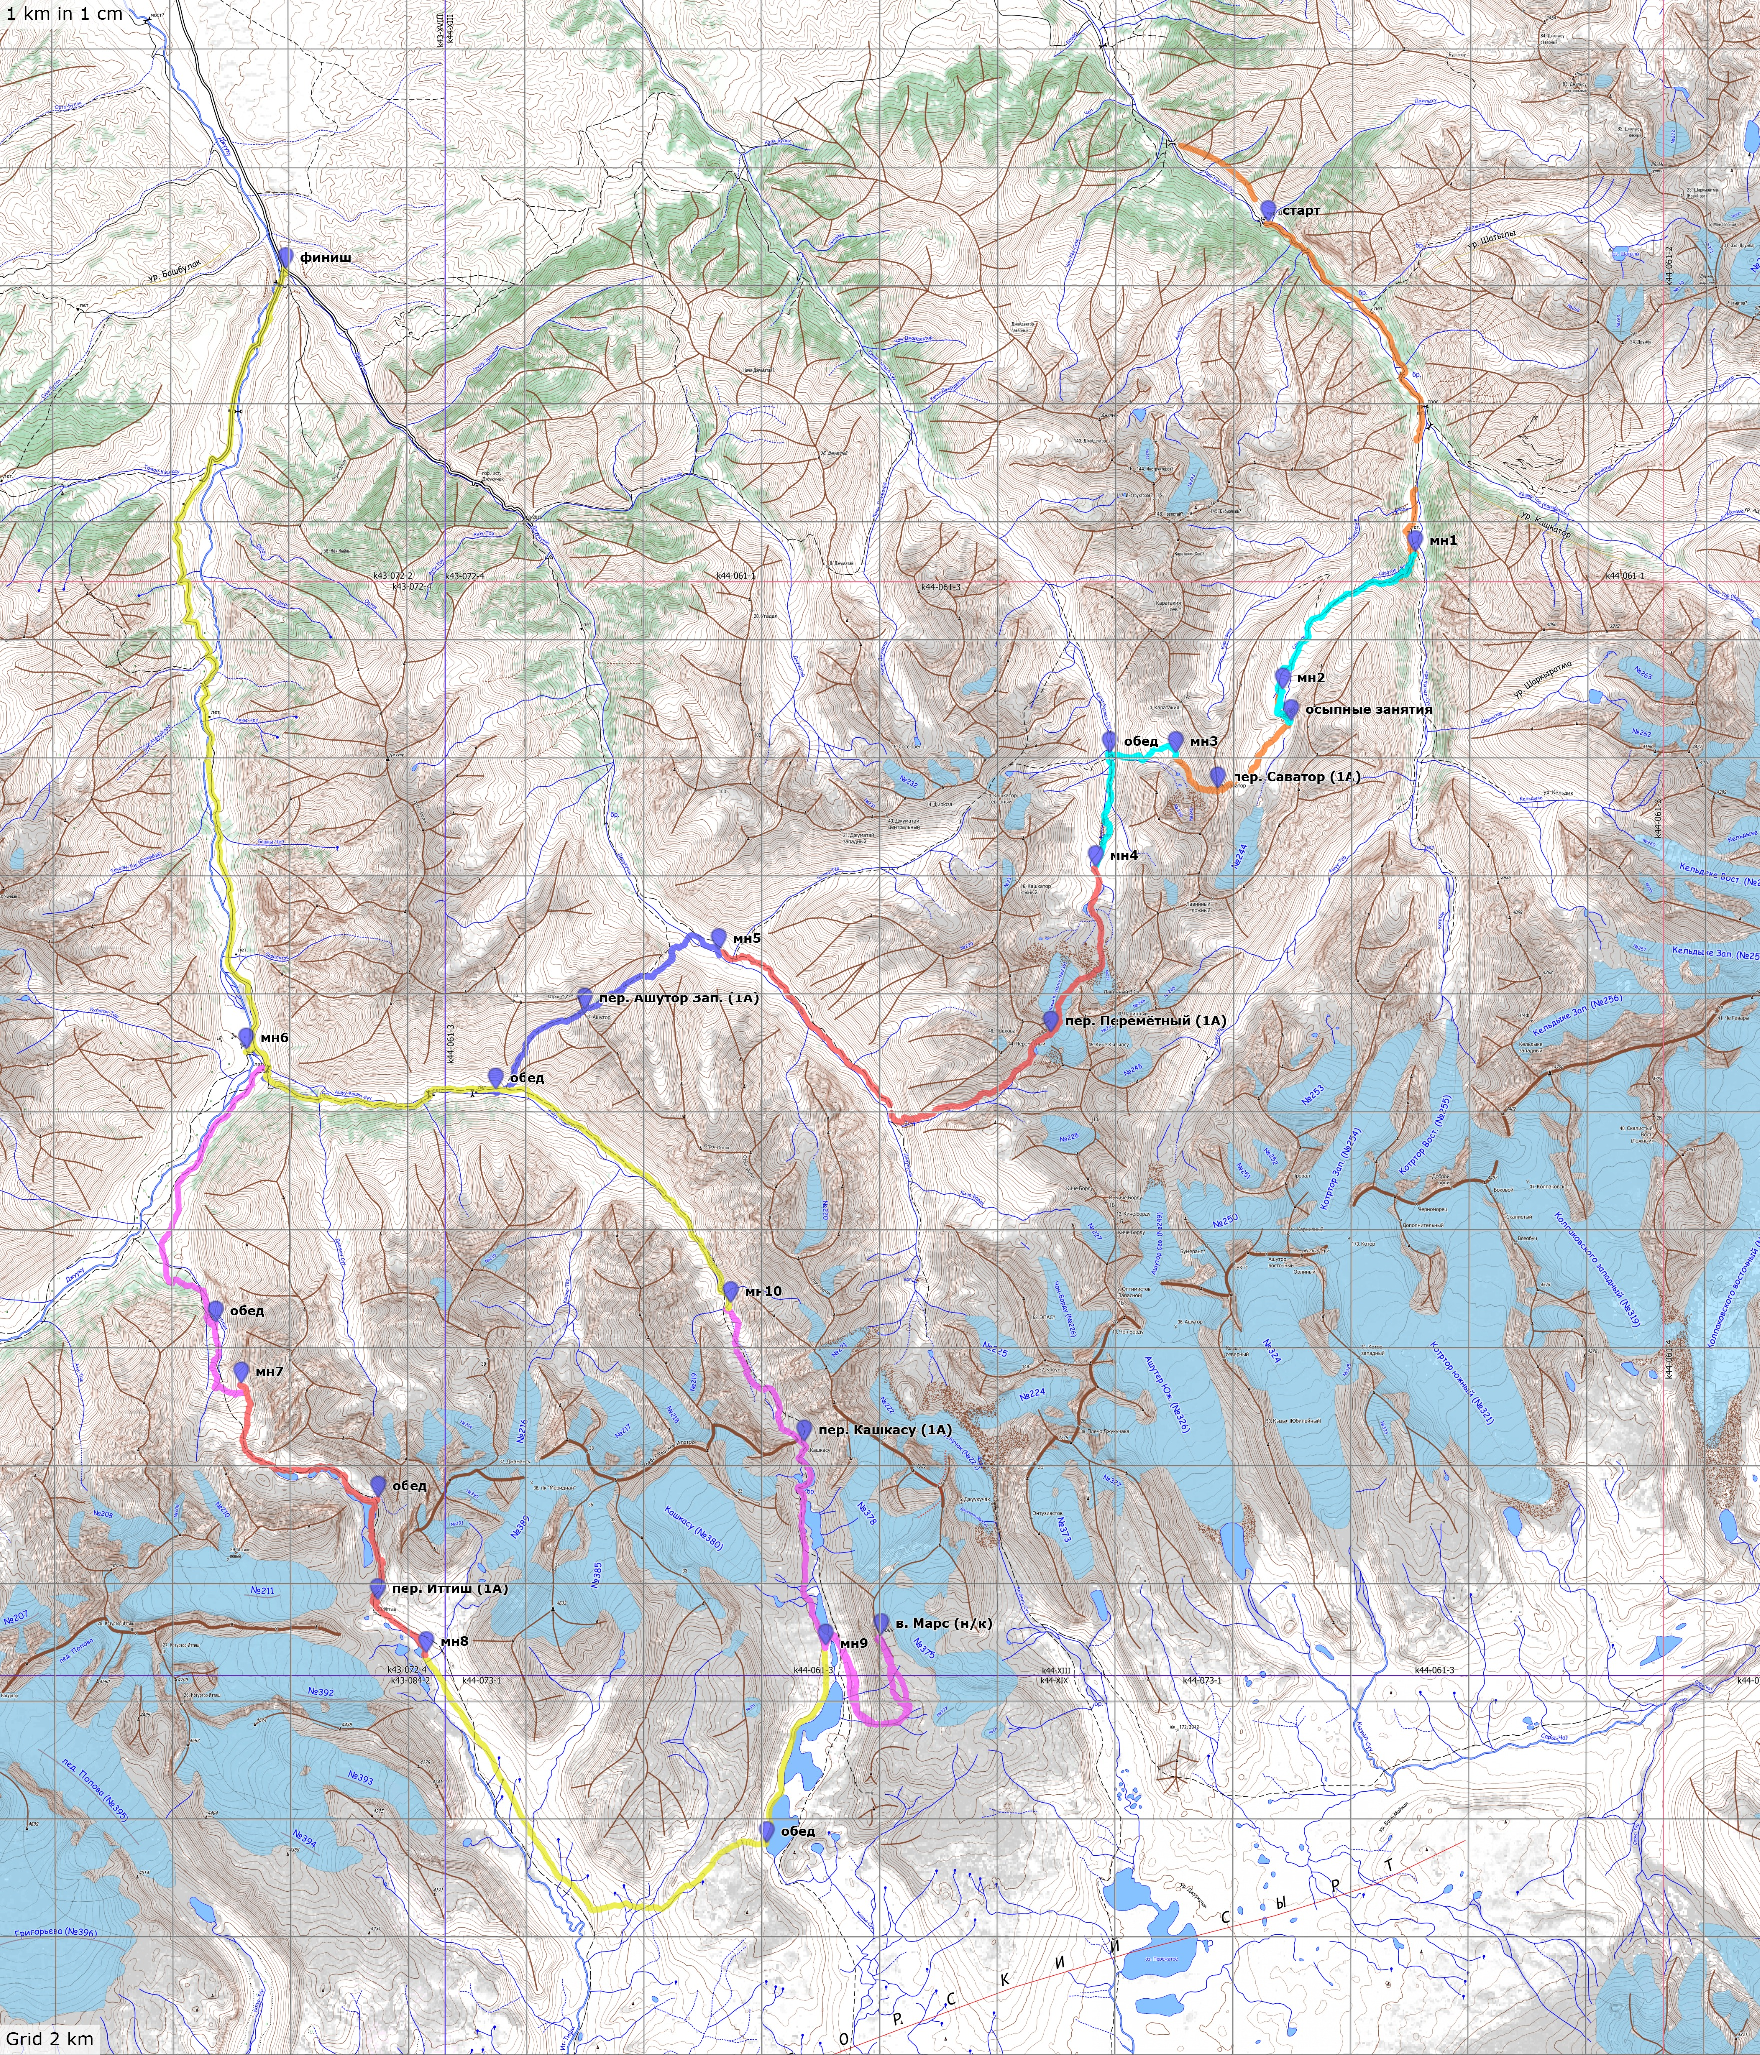
\includegraphics[width=0.7\linewidth]{pics/maps/map}
	\caption{Обзорная схема маршрута}
\end{figure}

\newpage
\subsection{Высотный профиль маршрута}

\begin{figure}[h!]
	\centering
	\includegraphics[width=0.92\linewidth]{pics/elevation_vs_time}
	\includegraphics[width=0.92\linewidth]{pics/elevation_vs_distance}
	\caption{Высотный профиль маршрута}
	\label{fig:heights}
\end{figure}

\newpage
\subsection{Расчёт к.с. маршрута}

\textbf{Протяжённость $\text{Lмар}$} маршрута (измерено на сайте nakarte.me с домножением на коэффициент $k=1.1$~согласно~\cite{method})~--- 92.0~км.

\textbf{Продолжительность $\text{T}$} маршрута~--- 7 дней.

\subsubsection{Локальные препятствия}
\textbf{Перевалы:} 6 н/к: $6\cdot2=12$~баллов (в зачёт \textbf{4 балла})

\textbf{Переправы:} 1 н/к: $1\cdot0.5=0.5$~баллов (в зачёт \textbf{0.5 балла})

Итого в зачёт \textbf{$\text{\textbf{ЛП}}=4.5$~балла.}

\subsubsection{Протяжённые препятствия}
\textbf{Коэффиициент трудности района:} $\text{Кт}=0.35$ (Западный Кавказ)

\textbf{Количество баллов за протяженные препятствия маршрута:} $\text{ППор}=12$

\textbf{Нормированная протяжённость маршрута 1 к.с.:} $\text{L}=100$~км

Итого в зачёт $\text{\textbf{ППб}}=\text{Кт}\cdot\text{ППор}\cdot\frac{\text{Lмар}}{\text{L}}=4.6$~\textbf{балла}.

\subsubsection{Интегральная оценка маршрута препятствия}

\textbf{Географический показатель района:} $\text{{Г}}=4$ (Западный Кавказ)

\textbf{Коэффициент перепада высот:} $\text{К}=1+\dfrac{\Delta H}{\text{В}}=1+\dfrac{8126}{12000}=1.7$

\textbf{Коэффициент автономности} в походах 1--2 к.с. принимается равным A=1.

Итого в зачёт $\text{\textbf{Рб}}=\text{Г}\cdot\text{К}\cdot\text{А}=8.4$~\textbf{балла}.

Итоговая сумма $\text{\textbf{КСб}}=\text{ЛПб}+ \text{ППб} + \text{Рб}=\mathbf{17.5}$~\textbf{баллов}, что соответствует походу 1 к.с. (7--20~баллов).

\clearpage
\subsection{Список участников} 

\begin{table}[h!]
	\centering
	\resizebox{0.99\textwidth}{!}{%
	\begin{tabular}{|>{\centering\arraybackslash}m{0.015\linewidth}|>{\centering\arraybackslash}m{0.2\linewidth}|>{\centering\arraybackslash}m{0.18\linewidth}|>{\centering\arraybackslash}m{0.05\linewidth}|>{\centering\arraybackslash}m{0.15\linewidth}|>{\centering\arraybackslash}m{0.3\linewidth}|}
		\hline
		\textbf{№} &
		\textbf{Фото} &
		\textbf{ФИО} &
		\textbf{г.р.} &
		\textbf{Обязанности в группе} &
		\textbf{Туристский опыт} \\
		\hline			
		
		1	&	\includegoogle[width=0.99\linewidth]{https://drive.google.com/file/d/1WISFuT9mIPXXT3c39rQQxuTZFQ0DJDx6/view}	& Остапив Алексей Юрьевич	&	1998	&	Руководитель, завхоз, носитель аптечки	& 1ГР, Терскей\newline2ГУ, Киргизский хребет,\newline 3$\times$1ГУ, Кавказ, Алтай \newline 2А тур., 1Б альп.\\
		\hline
		2	&	\includegoogle[width=0.99\linewidth]{https://drive.google.com/file/d/1rtFU66LaAsBDkXLVvV_-qe-KaqowPTdq/view}	&	Миронова Наталья Сергеевна	&	2000	&	Логист, финансист	&	2 ст.с.  Кавказ\newline 1А тур.\\
		\hline
		3	&	\includegoogle[width=0.99\linewidth]{https://drive.google.com/file/d/14mMi30ReTcrAUe4Hq6GsIjTiF4xvJbe7/view?usp=drive_link}	&	Гурский Артур Антонович	&	2003	&	Штурман, завснар, реммастер	&	1ГУ Терскей\newline1ПУ Крым\newline 1А тур.\\
		\hline
		4	&	\includegoogle[width=0.99\linewidth]{https://drive.google.com/file/d/1mPloHi0eN2j-M4MDuHpngwGsX-CevGd7/view?usp=drive_link}	&	Зернина Юлия Алексеевна	&	2004	&	Фотограф, хронометрист	&	1ГУ Терскей\newline 1А тур.\\
		\hline
		4*	&	\includegoogle[width=0.99\linewidth]{https://drive.google.com/file/d/1bN6RrMDDclIQesFk1KIZdMmjUpg2gKt6/view?usp=drive_link}	&	Йошта	&	2022	&	Талисман команды	&	1ГУ Кавказ\newline 1А тур.\\
		\hline
	\end{tabular}%
}
\end{table}


\clearpage
	\section{Организация и проведение похода}
\subsection{Цели и задачи маршрута. Выбор нитки маршрута}
Идеологическим вдохновителем и составителем нитки маршрута был не руководитель, а одна из участниц, Наташа Миронова. Сама идея погулять по осеннему Приэльбрусью возникла после майского н/к треккинга \cite{ostapiv2025}, когда из-за большого количества снега мы не смогли подняться ни на один перевал, равно как перевалить через юго-восточный отрог Эльбруса от водопада Терскол к водопаду Девичьи косы. Однако при детальной проработке маршрута захотелось уйти от большого количества раздробленных радиалок с логистикой между ними и пройти линейный маршрут. Первая его версия проходила через ряд перевалов 1А, таких как, например, Исламсу. Однако МКК нас предупредила, что в начале сентября на седловинах этих перевалов уже может лежать снег и, как следствие, горный поход будет считаться межсезоньем с соответствующими требованиями к опыту руководителя и участников. Поэтому и решили организовать пешеходный поход по некатегорийным перевалам. Фактически, мы <<изобрели>> стандартную нитку коммерческого маршрута из Хурзука в Верхний Баксан. Имея в ввиду вышесказанное, перечислю и побочные \textbf{цели}, которые были поставлены при планировании маршрута:

\paragraph{Посмотреть красивое.} Изюминкой маршрута стал вид на Эльбрус с нескольких сторон, водопады в Джилы-Су и пещеры горы Улkукая.

\paragraph{Погулять по невысоким горам.} Руководителю похода не доводилось раньше проводить поход по среднегорью, с его особенным ландшафтом~--- исправляем!
	
	
\paragraph{Сходить в горы осенью.} Возможность посмотреть на то, что такое осень в горах стала немаловажным фактором при выборе времени похода. К тому же мы надеялись на сухую ссентябрьскую погодав. Тем не менее, оказалось, что осень~--- это плачущее небе под ногами$\ldots$

\paragraph{Не упарываться.} Хотелось избежать технически сложных участков на маршруте, поскольку в этом сезоне для таких целей у нас был Тескей \cite{teskei2025ostapiv}, а также потому что некоторые участники группы не обладают достаточной квалификацией для преодоления их в межсезонье. Маршрут даёт возможность пройти простыми треккинговыми тропами.

В выборе района, конечно, огромную роль играла и простота логистики.

\subsection{Логистика}
Подьезд первой половины группы осуществлялся на поезде Москва---Кисловодск до станции Минеральные Воды (прибытие в 7:20). Оставшаяся половина группы добиралась до места на самолете Уральских авиалиний Москва---Минеральные Воды, рейс U6-153 (прибытие в 14:45). От Минеральных Вод до а. Хурзук добирались на трансфере, заказанном через Бориса Саракуева (+7(928)-950-38-68, +7(929)-884-31-75, bezonec@list.ru). Время движения~--- порядка 4 часов. Стоимость трансфера туда составила 12000~\faRub.~Обратно до Минеральных Вод добирались на трансфере, так же заказанном через Бориса Саракуева, из Верхнего Баксана. Время движения~--- 3 часа, стоимость~--- 10000~\faRub.

\subsection{Аварийные выходы из маршрута и его запасные варианты}
\textbf{Аварийными выходами} с маршрута являлось следование по его нитке до ближайшей цивилизации. В первые два дня таковым является движение обратно в сторону Хурзука, далее, от пер. Чемарт и до пер. Кыртыкауш~--- спуск в Джилы-Су, а далее~--- спуск в Верхний Баксан по д.р. Кыртык.


\textbf{Запасными вариантами} маршрута являлся отказ от прохождения пер. Сылтран и спуск по д.р. Кыртык в Верхний Баксан.


\subsection{Изменение маршрута и их причины}
Воспользовались запасным вариантом~--- отказ от прохождения пер. Сылтран и спуск в Верхний Баксан по д.р. Кыртык. Сделали это в связи с тем, что длительный спуск (около 2 км по вертикали) почти гарантированно привёл бы к проблемам с коленями у одного из участников. К тому же, судя по отзывам встреченных нами туристов, на седловине перевала уже лежал снег.

\subsection{Обеспечение безопасности на маршруте}
Группа была зарегистрирована в МЧС по КЧР и КБР (две заявки, отправленные за 4 дня до выхода на маршрут). На маршруте дежурные МЧС по КЧР просили предоставлять всю информацию о передвижении (старт, пересечение границы республик, финиш), причём, после того, как отзвонились из КБР, перевели нашу заявку в местное МЧС. Дежурный по КБР, наоборот, не просил отзваниваться, мотивируя тем, что необходимые даты указаны в заявке (а на финише удивлялся, откуда взялись две заявки; видимо, это произошло благодаря ретивым сотрудникам из КЧР). Номера дежурных: для КЧР: +7(878) 226-62-00, для КБР: +7(8662)742-556.

Для обмена сообщениями, отслеживания положения группы на карте, а также возможности экстренной связи, в группе имелся спутниковый треккер IRIDIUM Rockstar 360. Стоимость аренды треккера в компании <<Satellite-Rent>> составила 600~\faRub~в день, залог~--- 50000~\faRub, за услуги связи~--- 3780~\faRuble,~70~\faRub~за юнит. К сожалению, связь была плохой, точки не отправлялись, а сообщения смогли отправиться только несколько раз за поход. Тем не менее, наличие трекера было оправдано, ибо все-таки известия доходили и, что главное, из д.р. Кыртык смогли отправить координатору сообщение с просьбой перенести трансфер на два дня раньше, и к моменту нашего выхода на связь транспорт уже был организован.

Каждый участник самостоятельно оформлял на себя индивилуальный страховой полис. Выбрали страховую фирму <<Совкомбанк страхование>>, ассист AP Companies, размер страховой защиты 35000~USD,  вид отдыха <<Экстремальный отдых>>. Стоимость полиса составила 2012~\faRuble~с человека.

\subsection{Перечень наиболее интересных природных и исторических объектов, занятий на маршруте}
\begin{enumerate}[noitemsep,topsep=0pt,parsep=0pt,partopsep=0pt]
	\item Хребет Енукол~--- высокогорные степи;
	\item Эльбрус, который в этом походе можно было рассмотреть с трех сторон~--- с запада, севера и востока;
	\item Плато Ирахитсырт в Северном Приэльбрусье;
	\item Джилы-Су с его нарзанами, термальными источниками, Калиновым мостом и водопадо Султан;
	\item Скала Уллу-Кая в д.р. Кыртык (каменоломни, потрясающего видак скалы, нарзан).
\end{enumerate}

\paragraph{Темы практических занятий:}

\begin{itemize}
	\item Техника передвижения по травянистым и осыпным склонам;
	\item Техника несложных бродов поодиночке;
\end{itemize}

\newpage
\subsection{Развёрнутый график движения}
\alert{Артур, это на тебе, пожалуйста}
\begin{table}[h!]
	\centering
	\resizebox{0.95\textwidth}{!}{%
		\begin{tabular}{|>{\centering\arraybackslash}m{0.045\linewidth}
				|>{\centering\arraybackslash}m{0.02\linewidth}
				|>{\centering\arraybackslash}m{0.43\linewidth}
				|>{\centering\arraybackslash}m{0.09\linewidth}
				|>{\centering\arraybackslash}m{0.1\linewidth}
				|>{\centering\arraybackslash}m{0.05\linewidth}
				|>{\centering\arraybackslash}m{0.09\linewidth}
				|>{\centering\arraybackslash}m{0.13\linewidth}|}
			\hline						
			Дата	&	\begin{turn}{90}День\end{turn}	&	Участок маршрута	&	Км с $k=1.2$	&	Набор /сброс, м	&	ЧХВ	&	Высота ночёвки, м	&	Способы передвижения	\\
			\hline
			
			18.08	&	1	&	г.~Минеральные воды~--- аул Верхний Учкулан~--- д.р Учкулан~--- д.р. Кичкинакол Уллукёльский	&	5.3	&	$+650$\newline$-0$	& 2:46	&	2200	&	Машина,\newline Пешком	\\
			\hline
			19.08	&	2	&	д.р. Кичкинакол Уллукёльский~--- оз. Гитче-Кёль~--- оз. Уллу-Кёль 	&	5.6	& $+650$\newline$-0$		& 3:25		& 2850		&	Пешком	\\
			\hline
			20.08	&	3	&	м.н.~--- \textbf{пер. Уллу-Кёль Восточный (1А$^\star$, 3050)}~--- кош в д.р. Трёхозёрная~--- д.р. Махар	&	7.2	& $+200$\newline$-1190$		& 7:39	& 1860		&	Пешком	\\
			\hline
			21.08	&	4	&	м.н.~--- т/б <<Глобус>>~--- д.р. Гондарай~--- д.р. Джалпаккол	&	11.3	&$+390$\newline$-225$		& 3:54		& 2120		&	Пешком	\\
			\hline
			22.08	&	5	&	м.н.~--- д.р. Кичкинекол Джалпаккольский~--- м.н. под моренным валом пер. Джалпаккол Северный	&	5.8	& $+620$\newline$-0$		& 3:56	& 2740		&	Пешком	\\
			\hline
			23.08	&	6	&	м.н.~--- \textbf{пер. Джалпаккол Северный (1А$^\star$, 3411)}~--- зелёные ночёвки на спуске в д.р. Мырды	&	5.0 	& $+660$\newline$-395$		& 6:16		& 3015		&	Пешком	\\
			\hline
			24.08	&	7	&	м.н.~--- д.р. Мырды~--- а/л <<Узункол>>	&	7.5	& $+0$\newline$-960$		& 3:53		& 2060		&	Пешком	\\
			\hline
			25.08	&	8	&	м.н.~--- д.р. Кичкинекол~--- д.р. Таллычат~--- Поляна Крокусов	&	7.1	& $+780$\newline$-0$		& 3:23		& 2840		&	Пешком	\\
			\hline
			26.08	&	9	&	м.н.~--- \textbf{пер. Кичкинекол Малый (1А, 3206)}~--- д.р. Чунгур-Джар	&	4.6	& $+360$\newline$-520$		& 2:42		& 2680		&	Пешком	\\
			\hline
			27.08	&	10	&	м.н.~--- \textbf{пер. Перемётный (1А, 3255)}~--- д.р. Танышхан	&	7.1	& $+575$\newline$-935$		& 6:50		& 2320		&	Пешком	\\
			\hline
			28.08	&	11	&	м.н.~--- д.р. Чиринкол~--- д.р. Кубань &	12.7	& $+90$\newline$-500$		& 3:23		& 1890		&	Пешком	\\
			\hline
			29.08	&	12	&	м.н.~--- погранзастава <<Хурзук>>~(рад.)~--- д.р. Уллу-Кам	&	20.9	& $+1210$\newline$-370$		& 7:15		& 2725		&	Пешком	\\
			\hline
			30.08	&	13	&	м.н.~--- \textbf{пер. Хотютау (1А$^\star$, 3546)}~--- лед. Большой Азау~--- оз. Эльбрусское~--- ст. <<Старый Кругозор>>~--- поляна Азау & 10.9	& $+800$\newline$-615$		& 4:25		& 2915		&	Пешком, Канатная дорога	\\
			\hline
			\multicolumn{3}{|c|}{\textbf{\textit{\Large{Итого:}}}} & \large{\textbf{111.0}} & \large{$\mathbf{+6985}$\newline$\mathbf{-5210}$	}	& \multicolumn{3}{c|}{\large{\textbf{58:08}\newline\textbf{2д 10ч 08мин}}} \\
			\hline
		\end{tabular}
}	
	
\end{table}



\clearpage
%	\section{Литературный обзор по прохождению маршрута}

\subsection{Пер. Иттиш}

Пер. Иттиш ориентирован с севера на юг и является перевалом через основной хр. Тескей-Ала-Тоо. Это один из немногих перевалов через данный основной хребет, которые имеют (низкую) трудность 1А. Вообще говоря, пер. Иттиш~--- это выход на горизонтальное плато, на котором расположены сырты (заболоченные луга). Лишь северная сторона перевала имеет наклон. Ранее \alert{ссылка} перевал проходился на спуск с юга на север; в данном походе было решено преодолеть его на подъем с севера на юг. При подготовке использовались отчеты \alert{ссылки}.

Подъем на перевал можно разбить на две части: подъем по тропе по хвойному лесу и осыпи и горизонтальное движение по средней и крупной осыпи. Второй этап недлинный по расстоянию -- около 4-5 км -- но может занять много времени из-за трудности рельефа. В некоторых местах можно сойти с крупных камней и двигаться по пересохшему дну озер, находящихся вблизи осыпи. При подходе к седловине видно обледенелый пик Иттиш и ледник, примыкающий к нему. После взятия перевала спуска нет -- сразу идет выход на высокогорные сырты и озера. Также в хорошую погоду с седловины открывается вид на соседний хр. Акшийрак. В целом, подъем является постепенным и не имеет крутых взлетов.

Суммарный перепад высот от д.р. Джууку, из которой начинался подъем, до седловины перевала составляет около 1000м, поэтому было решено устроить ночевку в середине подъема на небольшом озере, находящимся выше границы леса. От м.н. ночевки на озере до седловины перевала был пройден остаток подъема по средней осыпи и затем преодолен упомянутый затяжной участок горизонтальной осыпи.

\clearpage
	\section{Техническое описание маршрута}
\textit{Примечание:} везде, если не оговорено иное, имеются в виду правые и левые берега рек \textbf{орографически}.

\textbf{Отчёт писали:} Лёша Остапив, Саша Рогозин
\subsection{03 августа. Старт}
\textit{Метеоусловия: }

\begin{figure}[h!]
	\centering
	\includegraphics[angle=0, width=0.4\linewidth]{pics/maps/3}
	\label{fig:mini_18}
\end{figure}



\clearpage
\subsection{07 августа. пер. Перемётный (1А)}
\textit{Метеоусловия: утром, днём ясно, с 15:00 по 19:00 пасмурно, дождь, ночью сильный дождь}

\begin{figure}[h!]
	\centering
	\includegraphics[angle=90, width=0.7\linewidth]{pics/maps/7}
	\label{fig:7}
\end{figure}

Подъём дежурных в 04:30, выход в 07:10. Движемся к левому берегу одного из притоков в сторону небольшого голубого озерца в течение 15 мин ЧХВ и подходим к подножию морен. Приток можно перейти по камням, некоторые участники переходят в бродовой обуви.

\begin{figure}[h!]
	\centering
	\includegraphics[width=0.7\linewidth]{pics/07/IMG_2778}
	\caption{Место брода и дальшейшее движение по морене}
	\label{fig:img2778}
\end{figure}

Далее забираемся на моренный вал, огибаем локальную возвышенность справа пхд (рис.~\ref{fig:img2778}) и следуем по локальному понижению в направлении цирка Лавинных перевалов в течение 30 мин ЧХВ. Уклон не более 15\degree, подниматься комфортно (рис.~\ref{fig:DJI_0059.jpg}).

\begin{figure}[h!]
	\centering
	\includegraphics[width=0.9\linewidth]{pics/07/DJI_0059.jpg}
	\caption{Маршрут подъёма на пер. Перемётный}
	\label{fig:DJI_0059.jpg}
\end{figure}

Выходим на левый пхд борт ледника с осыпного гребня, разделяющего цирки Лавинных перевалов и пер. Перемётный, поскольку подъём с языка ледника без кошек невозможен. Ледник открытый, пологий и проходится без кошек. Его уклон не превышает 10\degree, лишь в верхней его части есть участок крутизной до 15\degree и с поперечными трещинами, которые легко обходятся.

\begin{figure}[h!]
	\centering
	\includegraphics[width=0.9\linewidth]{pics/07/IMG_2857.jpg}
	\caption{Движение по леднику}
	\label{fig:IMG_2857.jpg}
\end{figure}

\begin{figure}[h!]
	\centering
	\includegraphics[width=0.9\linewidth]{pics/07/IMG_2904.jpg}
	\caption{Движение по леднику}
	\label{fig:IMG_2904.jpg}
\end{figure}

\begin{figure}[h!]
	\centering
	\includegraphics[width=0.9\linewidth]{pics/07/view_kiche.jpg}
	\caption{Маршрут подъёма, вид с седловины}
	\label{fig:view_kiche.jpg}
\end{figure}

\begin{figure}[h!]
	\centering
	\includegraphics[width=0.9\linewidth]{pics/07/DJI_0067.jpg}
	\caption{Группа на пер. Перемётный (1А). Вид в д.р. Джукучак}
	\label{fig:DJI_0067.jpg}
\end{figure}

\begin{figure}[h!]
	\centering
	\includegraphics[width=0.9\linewidth]{pics/07/DJI_0069.jpg}
	\caption{Группа на пер. Перемётный (1А). Вид в д.р. Киче-Кызыл-Суу}
	\label{fig:DJI_0069.jpg}
\end{figure}

Координаты сложенного нами тура: N 42.09765° E 78.12405°



\begin{figure}[h!]
	\centering
	\includegraphics[width=0.7\linewidth]{pics/07/IMG_3087.jpg}
	\caption{Спуск по крутому тр. склону в <<коридоре>> между обрывом и скальными  выходами}
	\label{fig:IMG_3087.jpg}
\end{figure}


В 16:50 спускаемся, наконец, на дно д.р. Джукучак и движемся вниз по долине в направлении ночёвок под пер. Ашутор Зап. Спустя 30 минут движения нас накрывает дождём. Решаем вставать на первых же удобных площадках и бродить р. Джукучак утром следующего дня. В итоге выбираем место за 600 м до брода через р. Джукучак. Первые участники подходят под м.н. в 18:30, ставят палатки и греют чай. Остальные подтягиваются к 19:00, поим всех чаем и раскладываем отдыхать. Дежурные также разносят еду по палаткам. Дождь к вечеру прекращается, однако ночью льёт пуще прежнего.
Координаты м.н.: N 42.11030° E 78.05595°. ЧХВ 10:14.

\clearpage
\subsection{9 августа. Подход под пер. Иттиш}
\textit{Метеоусловия: утром, днём, вечером ясно, тепло.}

Накануне участники, сошедшие с маршрута, забрали с собой, не считая личного снаряжения, 3 пары кошек, 3 ледоруба, тент и чуть меньше половины продуктов, рассчитанных на вторую часть похода. Вес рюкзаков у мужской части оставшихся участников в начале второй части похода составляет 25-27 кг.

\begin{figure}[h!]
	\centering
	\includegraphics[angle=0, width=0.7\linewidth]{pics/maps/9}
	\alert{карта}
	\label{fig:mini_9}
\end{figure}

Выходим с м.н. 5 на слиянии рек Джууку и Ашу-Кашкасу \alert{около 09:00}. Проходим вдоль р. Джууку по дороге по орогр. правому берегу и начинаем подъем вдоль ручья Иттиши по его орогр. левому берегу. Подъем идет по тропе по ельнику, угол наклона составляет 15-20\degree. В ходе подъема есть один крутой участок около 40м по перепаду высот, где тропа становится круче. Встаем на обед вблизи ручья \alert{в 12:30}.

\begin{figure}[h!]
	\centering
	\includegraphics[width=0.7\linewidth]{pics/09/IMG_3328}
	\caption{Тропа на подъеме на пер. Иттиш (вид сверху вниз)}
	\label{fig:IMG_3328}
\end{figure}

\begin{figure}[h!]
	\centering
	\includegraphics[width=0.7\linewidth]{pics/09/IMG_3346}
	\caption{Брод ручья и подъем к м.н. 6 по тр.-ос. склону}
	\label{fig:IMG_3346}
\end{figure}


После обеда начали движение в \alert{14:00}. Преодолели остаток подъема по лесу и вышли к средней осыпи. По ней еще поднялись на $\sim$100м, перешли ручей и, траверсируя с небольшим набором высоты осыпь и тр.-ос. склон, вышли к небольшому озеру. Встали на ночевку вблизи озера в \alert{17:30} на плановом м.н. 6. Координаты м.н. \alert{N \degree~E \degree}.


\begin{figure}[h!]
	\centering
	\includegraphics[width=0.7\linewidth]{pics/09/camp_09} % IMG_3357.JPG
	\caption{Место ночёвки 9-10.08}
	\label{fig:camp_09}
\end{figure}

\clearpage
\subsection{10 августа. Пер. Иттиш (1A)}
\textit{Метеоусловия: утром, днём, вечером ясно, тепло. В середине дня жарко.}

\begin{figure}[h!]
	\centering
		\includegraphics[angle=0, width=0.4\linewidth]{pics/maps/10}
	\label{fig:10}
\end{figure}

Подъем дежурных в 05:00, выходим с м.н. 6 в 07:15. К 10:30 преодолеваем подъем по морене и выходим на горизонтальную осыпь на высоте $\sim$3700м. Оставшуюся часть дня двигаемся по этой осыпи.

\begin{figure}[h!]
	\centering
	\includegraphics[width=0.7\linewidth]{pics/10/IMG_3429}
	\caption{Осыпь на подходе к пер. Иттиш}
	\label{fig:IMG_3429}
\end{figure}

Горизонтальная осыпь состоит из средних и крупных камней. В некоторых местах двигаемся по травянистым участкам, в некоторых~--- по пересохшей части дна озер, в некоторых приходится двигаться лазанием по крупным камням. Для ускорения рекомендуем ориентироваться на установленные туры, избегать лазания, пользоваться движением по дну озер, где это возможно. Однозначного рецепта преодоления данной осыпи нет.

\begin{figure}[h!]
	\centering
	\includegraphics[width=0.7\linewidth]{pics/10/IMG_3421}
	\caption{Движение по пересохшему дну озера}
	\label{fig:IMG_3421}
\end{figure}

В самое жаркое время суток, с 13:00 до 15:00, устраиваем обед вблизи ручья, впадающего в одно из озер (N 42.02672\degree~ E 77.98596\degree). После этого идём часть пути по дну озера и далее двигаемся по гребням морен. Морены состоят из камней среднего размера.

\begin{figure}[h!]
	\centering
	\includegraphics[width=0.7\linewidth]{pics/10/IMG_3489}
	\caption{Группа на седловине пер. Иттиш. Вид на сырты и хр. Акшийрак.}
	\label{fig:IMG_3489}
\end{figure}

На седловину перевала выходим в 17:00, преодолев кулуар, разделяющий моренный гребень с седловиной перевала. При движении по орогр. правому борту, по моренному карману, этот участок камнеопасен, так борт представлен отвесной стеной высотой несколько десятков метров~\cite{kovinov2021}. Однако при движении по гребню опасности поймать камень нет~\cite{tipsina2024} Спуска с перевала нет, сразу идет выход на высокогорные луга -- сырты. Пройдя по горизонтали около 1~км, встаём на ночевку на озере в 18:00, соединившись с группой Кати Тюриной. Координаты м.н.: N 42.00321\degree~ E 77.99574\degree.

\begin{figure}[h!]
	\centering
		\includegraphics[width=0.7\linewidth]{pics/10/camp_10}
	\caption{Место ночёвки 10-11.08}
	\label{fig:camp_10}
\end{figure}

\textbf{Выводы и рекомендации:} пер. Иттиш полностю соответствует заявленной к.тр. 1А. Определяющая сторона~--- северная. Перевал неклассический: перевальными взлётами не обладает, вместо этого с северной стороны~--- длительное движение по долине и широкому пологому кулуару с цепями озёр, а с южной~--- плоскогорье и сырты. Из-за последнего обстоятельства перевал необходимо включать в нитку маршрута не ранее середины похода, чтобы группа была акклиматизирована. Сам перевал необычен и красив из-за принципиальной возможности пересечь хребет Тескей-Ала-Тоо в горном походе 1 к.с., из-за открывающихся видов на сырты и высокие скальные гребни пересекаемого основного хребта. Горячо рекомендуется к посещению в новичковых горных походах.

\clearpage
%	\section{Материальное обеспечение группы}

\begin{table}[h!]
	\centering
	%	\resizebox{0.77\textwidth}{!}{%
		\begin{tabular}{|>{\centering\arraybackslash}m{0.02\linewidth}|>{\centering\arraybackslash}m{0.31\linewidth}|>{\centering\arraybackslash}m{0.08\linewidth}|>{\centering\arraybackslash}m{0.29\linewidth}|>{\centering\arraybackslash}m{0.08\linewidth}|}
			\hline
			\multirow{2}{*}{\textnumero}	&	\multicolumn{2}{|c|}{Общественное}	&	\multicolumn{2}{|c|}{Личное}	\\
			
			\cline{2-5} & Наименование	&	Кол-во	&	Наименование	&	Кол-во\\
			\hline
			1	&	Верёвка статическая 50~м	&	1	&	Каска	&	1	\\
			\hline
			2	&	Карабины	&	4	&	Ледоруб	&	1	\\
			\hline
			3	&	Жумар	&	1	&	Солнцезащитные очки	&	1	\\
			\hline
			4	&	Страховочная система	&	2	&	&	\\
			\hline
			5	&	Блокировка	&	2	&	&	\\
			\hline
			6	& Кошки	&	3	&	&	\\
			\hline
			7	&	Спусковое устройство	&	1	&	&	\\
			\hline
			8	&	Станционные петли	&	2	&	&	\\
			\hline
			9	&	Корделет	&	2	&	&	\\
			\hline
			10	&	GPS-навигатор	&	1	&	&	\\
			\hline
			11	&	Спутниковый телефон	&	1	&	&	\\
			\hline
			12	&	Рация*	&	1	&	& \\
			\hline
		\end{tabular}%
		%	}
\end{table}

* Вторая рация находилась у группы Е. Тюриной, проходившей похожий маршрут в то же время параллельно с нашей группой.



\clearpage
%	\section{Финансовый отчёт}

\begin{table}[htbp]
	\centering

		\begin{tabular}{|>{\centering\arraybackslash}m{0.5\linewidth}
				|>{\centering\arraybackslash}m{0.2\linewidth}
				|>{\centering\arraybackslash}m{0.2\linewidth}|}
			
			\hline						
		Статья расхода	&	На группу,~\faRub	&	На человека,~\faRub	\\
		\hline
		Поезд Москва--Мин. Воды	&	9852 	&	4926	\\
		\hline
		Самолёт Москва--Мин. Воды	&	21014	&	10507	\\
		\hline
		Поезд Мин. Воды--Москва	&	19968	&	4992	\\
		\hline
		Трансфер из Мин. Вод в Хурзук	&	12000	&	3000	\\
		\hline
		% 15 июля - 5 сентября
		Доставка забросок	&	10000	&	2500	\\
		\hline
		Хранение заброски в Джилы-Су	&	1000 & 250	\\
		\hline
		Трансфер из Верхнего Баксана в Мин. Воды & 10000 & 2500 \\
		\hline
		Ночёвка в а/л <<Лакколит>> & 2500 & 625 \\
		\hline
		Страховка & 6015 & 2005 \\
		\hline
		Аренда спутникового треккера & 13480 & 3370 \\
		\hline
		Продукты по раскладке и газ	&	8240	&	2060	\\
		\hline
		Прочее (хычины, вода на старте)	&	1040	&	260	\\
		\hline
		\textbf{ИТОГО:}	&	\textbf{115 109}	&	\textbf{28 777}	\\
		\hline
		\end{tabular}
	
\end{table}
% строка для того, чтобы git не ругался (я не знаю, почему он ругается)


\newpage
%	\section{Отчёт завхоза}

Продуктовая раскладка была позаимствована из августовского похода по Терскею \cite{teskei2025ostapiv} и несколько урезана. Именно, сыр на завтрак и хлебцы на обед и ужин были не каждый день, а через день. Граммовки сухмяса, пеммикана, суховощей были снижены на 20\%. Сделано это было с целью облегчения веса рюкзаков и поиска оптимума раскладки, т.к. в предыдущих походах, по мнению участников, раскладку можно было сделать <<тоще>>. Кроме того, имелось в виду, что физические нагрузки будут ниже, чем в обычной горной <<единичке>>

Что получилось в итоге:
\begin{itemize}
    \item По мнению одного участника из четырёх, раскладка была слишком <<тощей>>, хотя, по его же мнению, это можно было компенсировать более калорийной карманкой. Остальнм троим было приемлемо.
    \item С огромным удовольствием участники ели карпюр с пеммиканом и жареным луком: в одном кане на пеммикановом жиру жарится лук, в другом — 
	кипяток для разведения карпюра и чая.
	\item Чая много не бывает. На полуднёвках, под затяжной дождь, чай заходил очень хорошо.
    
\end{itemize}


%—————————————————————————————————————————————————
% С чего скатываю:
%Раскладка была составлено следующим образом: 
%− на завтрак были заложены гречка, булгур, рис, макароны или пюре (по 250г на 
%четверых) и 250 грамм тушеной свинины или говядины 
%− на обед брикетированный суп лидкон (гороховый, лидский, рассольник или харчо) 
%1 пачка 200г на четверых, 200г колбасы или паштета, 100г хлебцов 
%− на ужин заложены гречка, булгур, рис, макароны или пюре (по 250г на четверых), 
%325г тушеной говядины, тушеной свинины и 50г сала 
%− каждый прием пищи предполагал 4л чая 
%− на день выделялось 150г козинаков и 45г лимона 
%− каждому участнику на поход было выделено по 6 энергетических гелей GU Original 
%По результатам питания в походе можно сделать следующие выводы: 
%− главная проблема раскладки – однообразие. С учетом плохого аппетита во время 
%акклиматизации меню должно быть разнообразным и вкусным; 
%− супы лидкон не годятся к использованию в качестве единственного блюда на обед 
%каждый день; на вкус супы однообразны и быстро надоедают; к концу похода супы 
%не варили, на обед ограничивались колбасой/паштетом с хлебцами; 
%− тушенка «Кранидов» качественная и вкусная, но употребление ее два раза в день к 
%середине похода надоедает, поэтому включать в дневную раскладку ее стоит не 
%более раза; 
%− сладкого имеет смысл брать больше, козинаки съедали с удовольствием; 
%− самым вкусным блюдом, которое если все участники с удовольствием было пюре с 
%тушенкой 
%− энергетические гели произвели двоякое впечатление на участников – кому-то они 
%помогали восстанавливать силы, на кого-то не оказывали влияния совсем; 
%необходимо каждому участнику группы индивидуально до похода проверять 
%работоспособность таких гелей. 
% 
%В целом приходится отметить, что раскладка была недостаточно проработана. Главная 
%проблема – однообразие. Вероятно, такая раскладка была бы удовлетворительной без учета 
%влияния акклиматизации на аппетит, но для использования на высокогорных маршрутах ее 
%обязательно нужно переработать.

%	\section{Итоги похода, выводы и рекомендации по совершённому походу}

	\begin{enumerate}
		\item Одной из причин выбора сентября как месяца проведения похода была уверенность, что начало сентября не сильно отличается от конца августа в рамках погодных условий. Ожидалось, что будет сухо, солнечно и не дождливо. Тем не менее, во время похода часто шёл дождь, а примерно 7 сентября выше 3500 м появился снег. Это никак не повлияло на преодоление группой маршрута, но лишний раз подтвердило мнение, высказанное МКК, что даты похода уже стоит считать межсезоньем; % Не уверена, что это вывод, но упомянуть хочется.
		\item При планировании маршрута можно было закладывать гораздо большее расстояние, которое группа могла бы пройти за день. Особенно это чувствовалось в самом начале маршрута, когда движение осуществлялось по технически несложному хребту Енукол;
		\item Сам отказ от перевала Сылтран руководитель считает правильным решением, %Считает ведь, да?
		 потому что именно он дал возможность пройти интересный участок с пещерами. Они стали красивой финальной точкой в походе;
		\item Судя по комментариям участников, раскладку стоило сделать сытнее;
		\item Поскольку в группе было всего четыре участника, удельный вес общественного снаряжения на участника был велик. Как следствие, вырос вес рюкзаков, в сравнении с ожидаемым. В рамках этого маршрута наличие веревки и систем %По крайней мере, мне так показалось. Брод проходится без веревки, остальное - тоже.
		в общественном снаряжении является спорным вопросом;
		\item При подготовке к маршрутам, одной из целей которых является «посмотреть красивое» стоит узнавать интересные факты об этом самом «красивом». Иными словами, в этом походе хотелось бы видеть человека с должностью Краевед, который бы разведал, а потом рассказал, откуда взялись пещеры горы Улукая, почему Калинов мост проходит не через реку Смородину и что из себя представляет Немецкий аэродром с точки зрения истории;
		\item Решение, принятое касательно времени движения, считаю хорошим и правильным. Благодаря подьёмам в 4:00 -- 4:30 получалось захватить наибольшую часть хорошей погоды и был куда более широкий простор для выбора времени старта подходящего места ночёвки. Этот момент был плохо раскрыт в прошлых походах. % Тоже не уверена, нужно ли такое в выводах писать
		
		%% Комментарии про состав раскладки?
	\end{enumerate} 

	\clearpage
%	\section{Перевальные записки}

\begin{figure}[h!]
	\centering
	\includegoogle[width=0.7\linewidth]{https://drive.google.com/file/d/1TVdu_XKLAIgkT0yzovFTDI2sGHvlww4m/view?usp=drive_link}
	\caption{Записка с пер. Быкылы 1}
	\label{fig:bykyly1}
\end{figure}

\begin{figure}[h!]
	\centering
	\includegoogle[width=0.7\linewidth]{https://drive.google.com/file/d/1JJD5Z3uIjI0nPvWh9GMntdL7z19zH4wJ/view?usp=drive_link}
	\caption{Записка с пер. Быкылы 2}
	\label{fig:bykyly2}
\end{figure}

\begin{figure}[h!]
	\centering
	\includegoogle[width=0.7\linewidth]{https://drive.google.com/file/d/1IorUOghUqdaweMAUoZmiqHHnqr2W2M8i/view?usp=drive_link}
	\caption{Записка с пер. Чемарт}
	\label{fig:chemart}
\end{figure}

\begin{figure}[h!]
	\centering
	\includegoogle[width=0.9\linewidth]{https://drive.google.com/file/d/1iKenGW1xXVCUxCRVuut30HRMAkAJTI96/view?usp=drive_link}
	\caption{Записка с пер. Бурунташ}
	\label{fig:buruntash_front}
\end{figure}

\begin{figure}[h!]
	\centering
	\includegoogle[width=0.9\linewidth]{https://drive.google.com/file/d/1E_ZvZ2aRiUPNsWwPJ3H9p2N0hW8LTBjw/view?usp=drive_link}
	\caption{Записка с пер. Бурунташ}
	\label{fig:buruntash_rev}
\end{figure}

\begin{figure}[h!]
	\centering
	\includegoogle[width=0.5\linewidth]{https://drive.google.com/file/d/1Y4aSOYhgredlP8vphERZwTbr0WFg46Od/view?usp=drive_link}
	\caption{Записка с пер. Кыртыкауш}
	\label{fig:kyrtykaush}
\end{figure}


\clearpage
%	\appendix
	
	%\section{Перевальные записки}

\begin{figure}[h!]
	\centering
	\includegoogle[width=0.7\linewidth]{https://drive.google.com/file/d/1TVdu_XKLAIgkT0yzovFTDI2sGHvlww4m/view?usp=drive_link}
	\caption{Записка с пер. Быкылы 1}
	\label{fig:bykyly1}
\end{figure}

\begin{figure}[h!]
	\centering
	\includegoogle[width=0.7\linewidth]{https://drive.google.com/file/d/1JJD5Z3uIjI0nPvWh9GMntdL7z19zH4wJ/view?usp=drive_link}
	\caption{Записка с пер. Быкылы 2}
	\label{fig:bykyly2}
\end{figure}

\begin{figure}[h!]
	\centering
	\includegoogle[width=0.7\linewidth]{https://drive.google.com/file/d/1IorUOghUqdaweMAUoZmiqHHnqr2W2M8i/view?usp=drive_link}
	\caption{Записка с пер. Чемарт}
	\label{fig:chemart}
\end{figure}

\begin{figure}[h!]
	\centering
	\includegoogle[width=0.9\linewidth]{https://drive.google.com/file/d/1iKenGW1xXVCUxCRVuut30HRMAkAJTI96/view?usp=drive_link}
	\caption{Записка с пер. Бурунташ}
	\label{fig:buruntash_front}
\end{figure}

\begin{figure}[h!]
	\centering
	\includegoogle[width=0.9\linewidth]{https://drive.google.com/file/d/1E_ZvZ2aRiUPNsWwPJ3H9p2N0hW8LTBjw/view?usp=drive_link}
	\caption{Записка с пер. Бурунташ}
	\label{fig:buruntash_rev}
\end{figure}

\begin{figure}[h!]
	\centering
	\includegoogle[width=0.5\linewidth]{https://drive.google.com/file/d/1Y4aSOYhgredlP8vphERZwTbr0WFg46Od/view?usp=drive_link}
	\caption{Записка с пер. Кыртыкауш}
	\label{fig:kyrtykaush}
\end{figure}


\clearpage
	
	
	\printbibliography



\end{document}